<<<<<<< HEAD
\section{Μαθηματικοί Ορισμοί}
=======
\section*{Ορισμοί}
\addcontentsline{toc}{section}{Μαθηματικοί Ορισμοί}
>>>>>>> 952d2026e75be50b99d277e6534ea5537ff2dcfe
\newtheorem{definition}{Ορισμός}
\label{appendix:math_definitions}

\subsection{Συναρτήσεις ενεργοποίησης}
\subsubsection{Συνάρτηση argmax}
\label{definition:argmax}
Δεδομένων ενός τυχαίου συνόλου \(X\), ενός συνόλου \(Y\) και μιας συνάρτησης \(f: X\rightarrow Y\), το μέγιστο όρισμα, argmax, πάνω σε ένα υποσύνολο \(S \subseteq X\) ορίζεται ως
\[argmax_{S} \: f := \underset{x \in S}{argmax} f(x) := \{x \in S \: | \: f(s) \leq f(x)  \: \forall s \in S\} \]


Με άλλα λόγια, η συνάρτηση argmax είναι το σύνολο των σημείων \(x\) για τα οποία η \(f(x)\) παίρνει την μέγιστη τιμή της.

\begin{figure}[h]
	\centering
	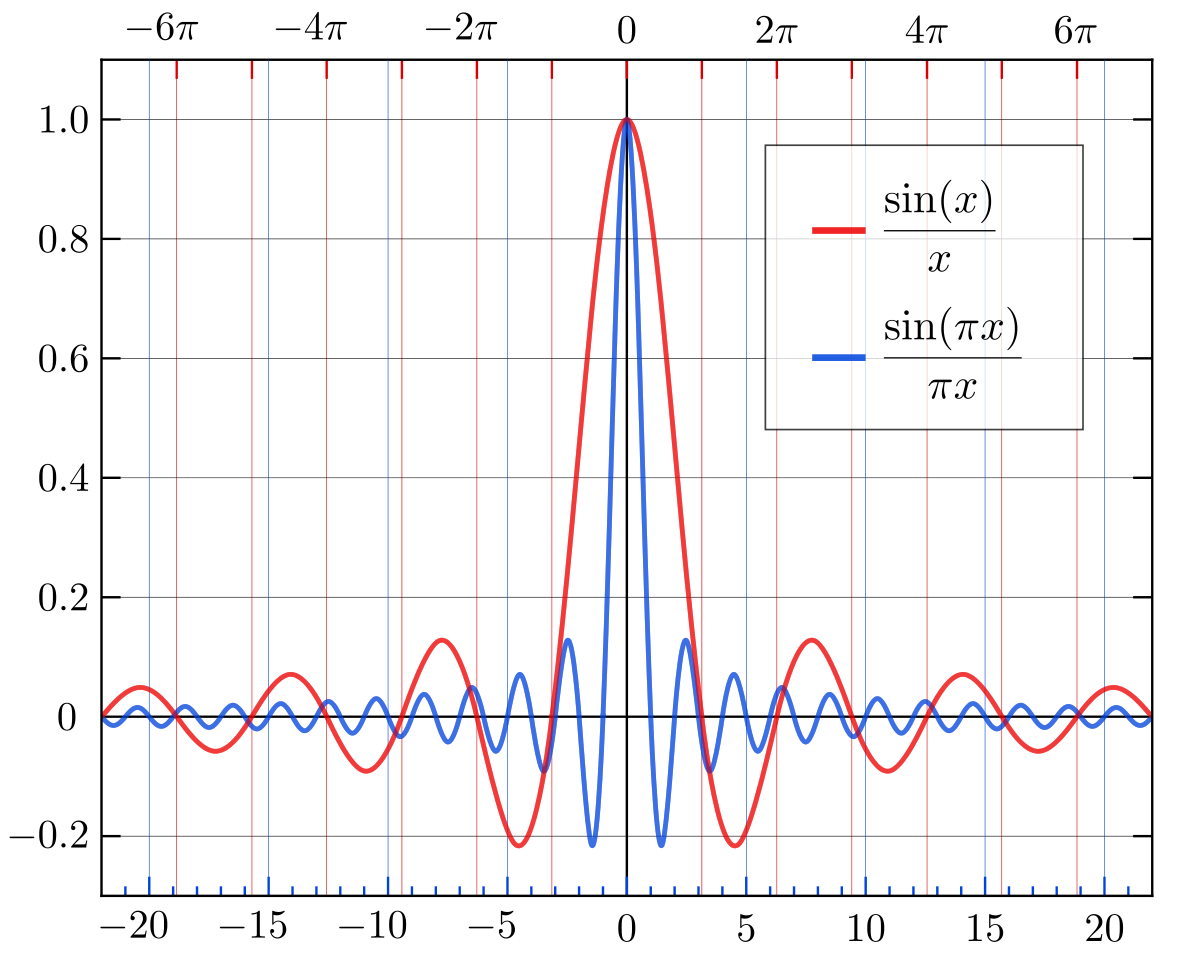
\includegraphics[scale=0.2]{images/appendix/function_argmax_example.png}
	\caption[Παράδειγμα συνάρτησης argmax]{Για παράδειγμα, οι συναρτήσεις \(sinc\) της γραφικής παράστασης έχουν και οι δύο \(argmax = 0\) επειδή έχουν στο \(x = 0\) μέγιστο το 1. }
\end{figure}


\subsubsection{Συνάρτηση soft-argmax}
\label{definition:soft-argmax}
Η συνάρτηση soft-argmax \(f: \mathbb{R}^K  \rightarrow [0, 1)^K\) ορίζεται όταν \(\lVert K \rVert > 1\) ως

\(soft\_argmax = \sigma(\boldsymbol{x})_i := \frac{e^{x_i}}{\sum_{j=1}^{K}e^{x_j}}\) για \(i = 1,\cdots,K\) και \(\boldsymbol{x} = (x_1,\cdots,x_K) \in \mathbb{R}^K \)


Ουσιαστικά, η συνάρτηση soft-argmax εφαρμόζει την κανονική εκθετική συνάρτηση σε κάθε στοιχείο \(x_i\) του διανύσματος \(\boldsymbol{x}\) και κανονικοποιεί τις τιμές διαιρώντας με το άθροισμα όλων των εκθετικών. Η κανονικοποίηση αυτή εξασφαλίζει ότι το άθροισμα των στοιχείων του διανύσματος εξόδου \(\sigma(\boldsymbol{x})\) είναι 1.

\subsubsection{Συνάρτηση ReLU}
\label{definition:relu}
Η συνάρτηση ReLU \(f: \mathbb{R} \rightarrow \mathbb{R}^+ \) ορίζεται ως

\( f(x) = max(0, x) \)

Δηλαδή, η συνάρτηση έχει ως έξοδο το όρισμα της όταν \(x > 0\), ενώ όταν \(x \leq 0\) η έξοδος είναι 0.

\begin{figure}[h]
	\centering
	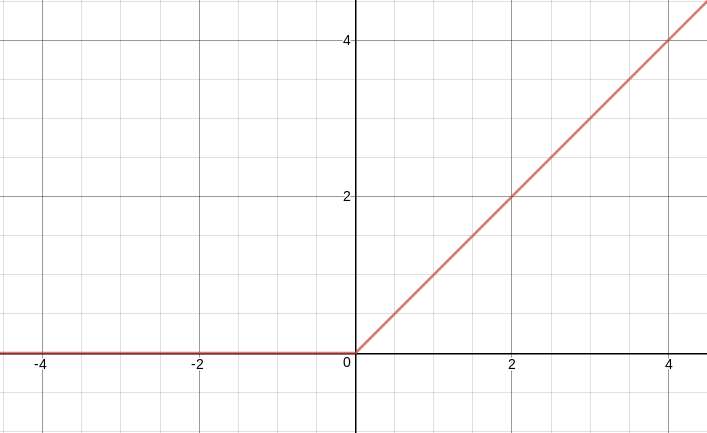
\includegraphics[scale=0.5]{images/appendix/relu_function.png}
	\caption{H συνάρτηση ReLU}
\end{figure}

\subsection{Επίπεδα νευρωνικών δικτύων}
\label{sec:nn_layers}

\subsubsection{Επίπεδο Fully Connected}

	Έστω το διάνυσμα εισόδου $ \pmb{x} \in \mathbb{R}^N $ ενός πλήρως συνδεδεμένου επιπέδου (fully connected layer) με $ N $ κόμβους εισόδου. Τότε, η έξοδος του $i$ κόμβου, $y_i \in \mathbb{R}$, θα δίνεται από
	
	\[ y_i(\pmb{x}) = f(\sum_{j=1}^N w_{ij}x_i + w_{i0} ) \]

	Ουσιαστικά, κάθε κόμβος εφαρμόζει έναν γραμμικό μετασχηματισμό στο διάνυσμα εισόδου μέσω του γινομένου του με τον πίνακα βαρών. Στο άθροισμα προστίθεται ένας σταθερός όρος ανά κόμβο το bias $w_{i0}$. Τέλος, στο αποτέλεσμα εφαρμόζεται ένας ενδεχομένως μη-γραμμικός μετασχηματισμός μέσω της συνάρτησης ενεργοποίησης $f$.

	\begin{figure}[H]
	\centering
	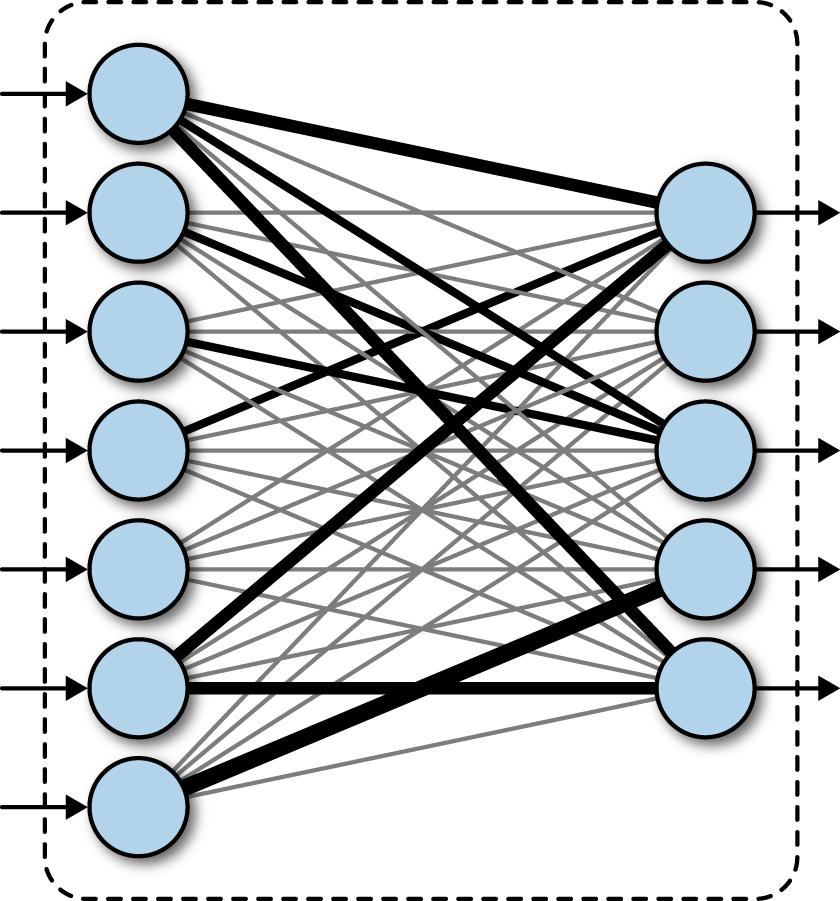
\includegraphics[scale=1]{images/appendix/fully_connected_layer.png}
	\caption[Επίπεδο Fully Connected]{\textsl{Επίπεδο Fully Connected}. Στο σχήμα φαίνεται ένα πλήρως συνδεδεμένο επίπεδο όπου όλοι οι κόμβοι εισόδου συνδέονται με όλους του κόμβους εξόδου. Οι ακμές με ποιο έντονο χρώμα υποδηλώνουν μεγαλύτερος βάρος μεταξύ του κόμβου εισόδου και εξόδου.}
	\label{fig:pooling_example}
\end{figure}

\subsubsection{Επίπεδο Batch Normalization}
\label{definition:batch_normalization}
	Η κανονικοποίηση παρτίδας (batch normalization) είναι μία μέθοδος στα νευρωνικά δίκτυα για την παραγωγή πιο γρήγορων και σταθερών αποτελεσμάτων. Η κανονικοποίηση παρτίδας στην είσοδο του κάθε επιπέδου γίνεται με την προσαρμογή της μέσης τιμής και της διακύμανσης των δεδομένων της παρτίδας, κατά την διαδικασία της εκπαίδευσης.
	
	Έστω ότι $B$ είναι μία παρτίδα μεγέθους $m$ δεδομένων. Τότε, η εμπειρική μέση τιμή και διακύμανση της $B$ θα είναι:
	
	\[ \mu_B = \dfrac{1}{m} \sum_{i=1}^{m} x_i \text{ και } \sigma_B^2 = \dfrac{1}{m} \sum_{i=1}^m(x_i - \mu_B)^2  \]
	
	Για ένα επίπεδο του δικτύου με είσοδο διαστάσεων $d$, $\pmb{x} = (x^{(1)}, \dots, x^{(d)})$, κάθε διάσταση της εισόδου κανονικοποιείται ξεχωριστά,
	
	\[ \hat{x}_i^{(k)} = \dfrac{x_i^{(k)} - \mu_B^{(k)}}{\sqrt{\sigma_B^{(k)^{2}} + \epsilon}} \text{ , όπου } k \in [1,d] \text{ και } i \in [1,m] \]
	
	Η $x_i^{(k)}$ και $\sigma_B^{(k)^{2}}$ είναι η ανά διάσταση μέση τιμή και διακύμανση αντίστοιχα. Το $\epsilon$ στον παρανομαστή είναι μία αυθαίρετη μικρή σταθερά για αριθμητική σταθερότητα.
	
	Η τελική κανονικοποιημένη είσοδος $\hat{x}_i^{(k)}$ έχει μηδενική μέση τιμή και μοναδιαία διακύμανση, αν δεν λάβουμε υπόψη το $\epsilon$. Για να αποκατασταθεί η αναπαραστατική ικανότητα του δικτύου, ένα βήμα μετασχηματισμού ακολουθεί
	
	\[ y_i^{k} = \gamma^{(k)}\hat{x}_i^{(k)} + \beta^{(k)} \]
	όπου οι παράμετροι $\gamma^{(k)}$ και $\beta^{(k)}$ μαθαίνονται κατά την εκπαίδευση.
	
	Επίσημα, η διαδικασία που υλοποιεί την κανονικοποίηση παρτίδας είναι ο μετασχηματισμός $BN_{\gamma^{(k)},\beta^{(k)}}: x_{1 \dots m}^{(k)} \rightarrow y_{1 \dots m}^{(k)}$, ονομαζόμενος Batch Normalizing transform. Η έξοδος του μετασχηματισμού $y^{(k)} = BN_{\gamma^{(k)},\beta^{(k)}}(x^{(k)})$ περνάει στα επόμενα επίπεδα του δικτύου, ενώ η κανονικοποιημένη είσοδος $\hat{x}_i^{(k)}$ παραμένει εσωτερικά του επιπέδου κανονικοποίησης παρτίδας.
		


\subsubsection{Επίπεδο Dropout}
\label{definition:dropout}
	Το επίπεδο Dropout των νευρωνικών δικτύων είναι μία μέθοδος ελάττωσης της υπερπροσαρμογής (overfitting) στα δεδομένα. Αυτό πετυχαίνεται παραλείποντας κόμβους είτε εμφανής είτε κρυμμένους κατά την διαδικασία της εκπαίδευσης.
	
	Για παράδειγμα σε ένα απλό πλήρως συνδεδεμένο γραμμικό επίπεδο η έξοδος περιγράφεται από
	
	\[ y_i = \sum_j w_{ij}x_j \text{ ή σε μορφή διανυσμάτων } \pmb{y} = \pmb{W}\pmb{x}\]
	
	όπου $y_i$ η έξοδος του κόμβου $i$, $w_{ij}$ τα βάρη πριν από το επίπεδο dropout και $x_j$ η είσοδος από τον κόμβο $j$.
	
	Η έξοδος του επιπέδου dropout ορίζεται ως
	
	\[ \pmb{\hat{w}}_j = 
		\begin{cases}
			\pmb{w}_j, \text{ με } P(c)\\
			\pmb{0}, \text{ διαφορετικά}
		\end{cases}	
	\]
	
	όπου $P(c)$ η πιθανότητα να παραμείνει η γραμμή του πίνακα βαρών. 
	
	Με άλλα λόγια, το επίπεδο dropout μηδενίζει τυχαία κάποιους κόμβους του προηγούμενου επιπέδου. Η διαδικασία που το πετυχαίνει αυτό, θέτοντας τα βάρη ίσα με το μηδέν, αφαιρώντας εξολοκλήρου τον κόμβο ή με κάποιον άλλον τρόπο, δεν επηρεάζει το τελικό αποτέλεσμα.
	
\subsubsection{Επίπεδο Convolution}
	\label{definition:convolution}

Το convolution επίπεδο χρησιμοποιείται κατά κόρων σε διεργασίες υπολογιστικής όρασης καθώς είναι άκρως αποδοτικό στην επεξεργασία εικόνων και στην εξαγωγή χαρακτηριστικών από αυτές. Η επεξεργασία γίνεται χωρικά πάνω στην εικόνα συλλαμβάνοντας έτσι αλληλεξαρτήσεις των πίξελ. Επιπλέον, απαιτεί μικρό αριθμό παραμέτρων και τα βάρη είναι επαναχρησιμοποιήσιμα βελτιώνοντας σημαντικά την εκπαίδευση.

Στο συνελικτικό επίπεδο (convolution layer) ένα φίλτρο ή πυρήνας περνάει διαδοχικά πάνω από τα 2D δεδομένα εισόδου, όπως φαίνεται στο Σχήμα \ref{fig:convolution_example}, πολλαπλασιάζοντας ανά στοιχείο τα στοιχεία του πίνακα στην συγκεκριμένη θέση και αθροίζοντας τα. Με αυτόν τον τρόπο, η αρχική εικόνα ή χάρτης χαρακτηριστικών μετατρέπεται σε έναν διαφορετικό χάρτη χαρακτηριστικών μικρότερων διαστάσεων, καθιστώντας πιο εύκολη και γρήγορη την επεξεργασία του.

\begin{figure}[H]
	\centering
	\label{fig:convolution_example}
	\begin{subfigure}[h]{0.45\textwidth}
		\centering
		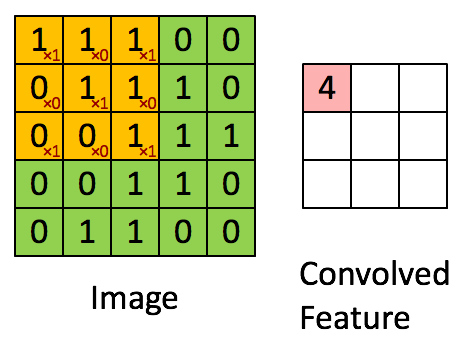
\includegraphics[width=\textwidth]{images/appendix/convolution_1.png}
		\caption{Η θέση του πυρήνα φαίνεται με κίτρινο χρώμα και με κόκκινη γραμματοσειρά οι τιμές του σε κάθε στοιχείο. Για τον υπολογισμό του χάρτη χαρακτηριστικών γίνεται πολλαπλασιασμός ανά στοιχείο και άθροιση.}
	\end{subfigure}
	\hfill
	\begin{subfigure}[h]{0.45\textwidth}
		\centering
		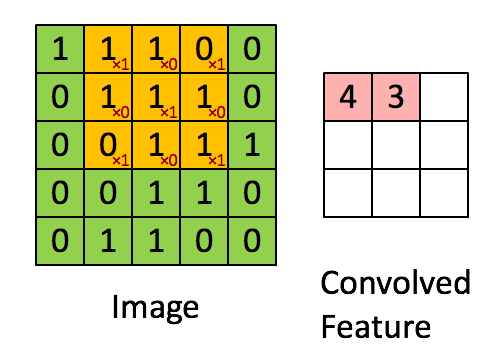
\includegraphics[width=\textwidth]{images/appendix/convolution_2.png}
		\caption{Στη συνέχεια, ο πυρήνας κινείται κατά μια θέση δεξία. Θα συνεχίσει να κινείται πάνω από τα δεδομένα εισόδου μέχρι να σαρώσει όλη την περιοχή.}
	\end{subfigure}
	\caption{Αριθμητικό παράδειγμα συνελικτικού επιπέδου}
\end{figure}

Φυσικά, κάποια χαρακτηριστικά της εικόνας χάνονται σε αυτή την διαδικασία. Εντούτοις, τα κύρια χαρακτηριστικά που είναι απαραίτητα για την πρόβλεψη του δικτύου διατηρούνται καθώς το δίκτυο κατά την εκπαίδευση έχει βελτιστοποιήσει τις παραμέτρους των απαιτούμενων φίλτρων για την διεξαγωγή της πρόβλεψης.

\subsubsection{Επίπεδο Pooling}
\label{definition:pooling}
	Αντίστοιχα με το convolution επίπεδο, ο σκοπός του επιπέδου pooling είναι να μειώσει το χωρικό μέγεθος του χάρτη χαρακτηριστικών. Τοιουτοτρόπως, μειώνοντας τις διαστάσεις επιτυγχάνεται μείωση της υπολογιστικής ισχύς που απαιτείται για την επεξεργασία των δεδομένων. Επιπλέον, είναι χρήσιμο στην εξαγωγή των επικρατέστερων χαρακτηριστικών που είναι αμετάβλητα κατά την περιστροφή και μετακίνηση, βελτιώνοντας έτσι την απόδοση της εκπαίδευσης.
	
	Υπάρχουν δύο είδη επιπέδων pooling, το max pooling και το average pooling, όπως φαίνεται στο Σχήμα \ref{fig:pooling_example}. Στην περίπτωση του max pooling, η έξοδος σε κάθε θέση του πυρήνα είναι το μέγιστο, ενώ στο average pooling η έξοδος σε κάθε θέση είναι ο μέσος όρος των στοιχείων που καλύπτονται από τον πυρήνα.
	
	\begin{figure}[H]
		\centering
		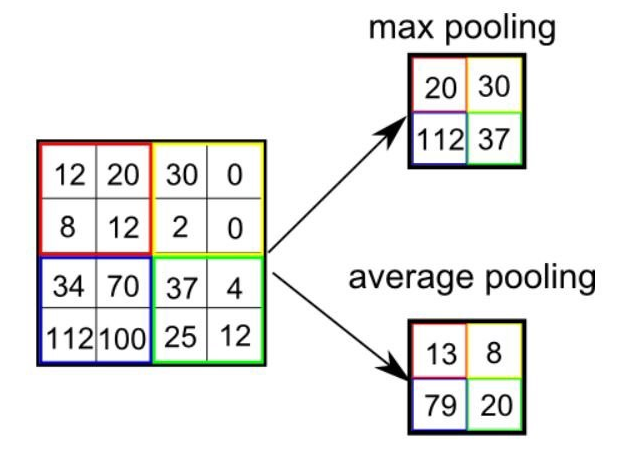
\includegraphics[scale=0.5]{images/appendix/pooling_example.png}
		\caption[Τύποι επιπέδων pooling]{\textsl{Τύποι επιπέδων pooling}. Στο σχήμα φαίνεται η έξοδος των επιπέδων max pooling (πάνω δεξιά) και average pooling (κάτω δεξιά) όταν τα δεδομένα εισόδου είναι ο πίνακας στα αριστερά. Σημειώνεται ότι ο πυρήνας και στις δύο περιπτώσεις κινείται πάνω στα δεδομένα με βήμα 2.}
		\label{fig:pooling_example}
	\end{figure}

\subsection{Υπόλοιπα}

\subsubsection{Κατευθυνόμενος Άκυκλος Γράφος}
	\label{definition:directed_acyclic_graph}
	Ένας γράφος ονομάζεται κατευθυνόμενος άκυκλος γράφος αν είναι κατευθυνόμενος και δεν περιέχει κύκλους. Με άλλα λόγια, αποτελείται από ακμές και κόμβους, με κάθε ακμή να κατευθύνεται από έναν κόμβο σε κάποιον άλλο, ενώ ταυτόχρονα ακολουθώντας τις κατευθύνσεις δεν δημιουργείται ποτέ ένας κλειστός βρόγχος. Δηλαδή για κανένα κόμβο δεν υπάρχει μονοπάτι (πέρα από το τετριμμένο) που να ξεκινά από αυτόν και να καταλήγει σ' αυτόν.
	
	Ένας κατευθυνόμενος γράφος είναι άκυκλος αν και μόνο αν μπορεί να ταξινομηθεί τοπολογικά, τοποθετώντας τους κόμβους σε μία γραμμική διάταξη όντας σύμφωνη με τις κατευθύνσεις των ακμών, όπως φαίνεται στο παράδειγμα του Σχήματος \ref{fig:directed_acyclic_graph}.
	
\begin{figure}[H]
	\centering
	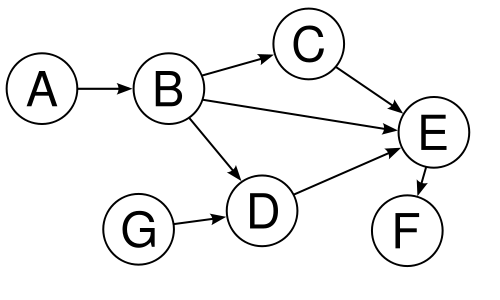
\includegraphics[scale=0.5]{images/appendix/directed_acyclic_graph.png}
	\caption{Παράδειγμα κατευθυνόμενου άκυκλου γράφου}
	\label{fig:directed_acyclic_graph}
\end{figure}


\subsubsection{Κατακόρυφο διάνυσμα κορυφής}
\label{definition:vertex_normal}

Στη γεωμετρία των γραφικών υπολογιστών, το κανονικό διάνυσμα κορυφής (\textsl{vertex normal}) σε μια κορυφή ενός πολυέδρου είναι το ευκλείδειο διάνυσμα κατεύθυνσης, προοριζόμενο ως αντικατάσταση του γεωμετρικού διανύσματος κάθετο στην επιφάνεια. Συνήθως, υπολογίζεται ως ο κανονικοποιημένος μέσος όρος των κάθετων διανυσμάτων επιφάνειας των πλευρών που περιέχουν την κορυφή, όπως φαίνεται στο Σχήμα \ref{fig:vertex_normal}. Τα vertex normals χρησιμοποιούνται για τον υπολογισμό της αντανάκλασης του φωτός όπως φαίνεται στο Σχήμα \ref{fig:vertex_normal_reflection}.

\begin{figure}[h]
	\label{fig:vertex_normal}	
	\centering
	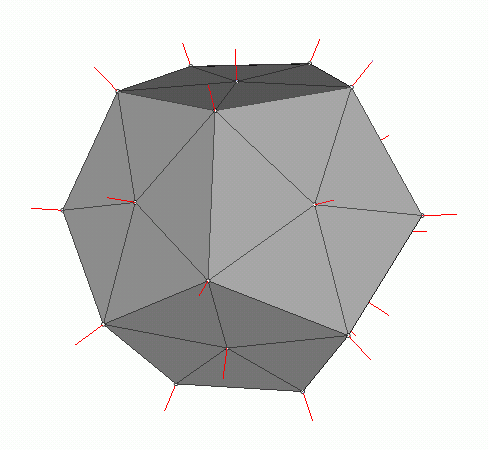
\includegraphics[scale=0.5]{images/appendix/vertex_normal.png}
	\caption[Κάθετα διανύσματα κορυφών πολύεδρου]{Τα κάθετα διανύσματα ενός δωδεκαέδρου πλέγματος σε κάθε κορυφή των τριγώνων που το απαρτίζουν.}
\end{figure}

\begin{figure}[h]
	\label{fig:vertex_normal_reflection}	
	\centering
	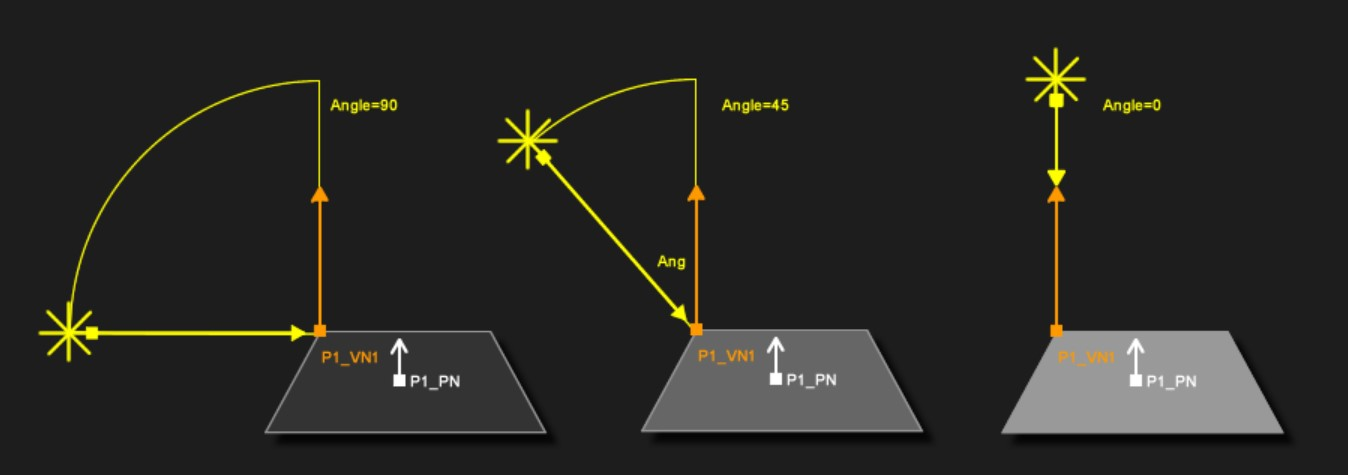
\includegraphics[scale=0.7]{images/appendix/vertex_normal_reflection.jpg}
	\caption[Αντανάκλαση του φωτός στο κάθετο διάνυσμα]{Καθώς η γωνία μεταξύ του διανύσματος φωτός και του vertex normal τείνει προς το μηδέν ο φωτισμός που δέχεται η κορυφή αυξάνεται στο μέγιστο. Αυτή η αρχή είναι η βάση όλων των υπολογισμών τρισδιάστατης σκίασης και δείχνει την σημαντικότητα των vertex normals.}
\end{figure}
